\documentclass[prd,amssymb,amsmath,amsfonts,nofootinbib,reprint,showpacs, longbibliography]{revtex4-1}

\usepackage{graphicx}
\usepackage{lmodern}
\usepackage{amsmath,amssymb}
\usepackage{mathrsfs}
\usepackage{amsfonts}
\usepackage[utf8]{inputenc}
\usepackage{url}
\usepackage[colorlinks]{hyperref}
\usepackage[dvipsnames]{xcolor}
\usepackage{multirow}
\usepackage[normalem]{ulem}
\usepackage{lipsum}

\usepackage{marvosym}
\usepackage{enumerate}
\usepackage{color,soul}

\usepackage{bm}
\usepackage{color}
\usepackage{commath}
\allowdisplaybreaks
\usepackage{multirow}

\def\lm{{\ell m}}

\def\TEOBResumS{\texttt{TEOBResumS}}
\def\TEOBResumSGIOTTO{\texttt{TEOBResumSGIOTTO}}
\def\TEOBResumSecce{\texttt{TEOBResumSecce}}
\def\bajes{\texttt{bajes}}
\def\Boldtheta{\boldsymbol{\theta}}
\def\Boldd{\textbf{d}}

\definecolor{cyan}{rgb}{0,0.9,0.9}
\definecolor{orange}{rgb}{0.9,0.5,0}
\definecolor{magenta}{rgb}{1,0,1}
\definecolor{purple}{rgb}{0.8,0.4,0.8}
\definecolor{gray}{rgb}{0.8242,0.8242,0.8242}
\definecolor{dodgerblue}{rgb}{0.12, 0.56, 1.0}

\newcommand{\AB}[1]{{\textcolor{violet}{{AB: #1}} }}
\newcommand{\RG}[1]{{\textcolor{dodgerblue}{{RG: #1}} }}
\newcommand{\MB}[1]{{\textcolor{purple}{{MB: #1}} }}
\newcommand{\AN}[1]{{\textcolor{magenta}{{AN: #1}} }}
\newcommand{\PS}[1]{{\textcolor{teal}{{PS: #1}} }}
\newcommand{\GP}[1]{{\textcolor{cyan}{{GP: #1}} }}

\newcommand{\todo}[1]{\textcolor{orange}{\texttt{TODO: #1}}} 
\newcommand{\red}[1]{\textcolor{red}{#1}} 
\newcommand{\bl}[1]{\textcolor{blue}{#1}} 
\newcommand{\cor}[2]{\sout{#1}\textcolor{red}{#2}} 
\newcommand{\old}[1]{\textcolor{gray}{\sout{#1}}}
\newcommand{\new}[1]{\red{#1}}


\begin{document}

\title{A very high impact paper about interesting things}
\author{Rossella \surname{Gamba}${}^{1}$}
\affiliation{${}^{1}$ Theoretisch-Physikalisches Institut, Friedrich-Schiller-Universit{\"a}t Jena, 07743, Jena, Germany}


\begin{abstract}
Paper template and related tools to ease arXiv submission.
\end{abstract}
\date{\today}
\maketitle

\section{Introduction}

\lipsum[1] \cite{2021arXiv210316737M}

%% Test if comments are removed

%% Test if figures are correctly labeled
\begin{figure}[t]
  \label{fig:duck}
    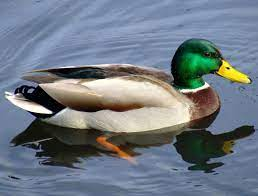
\includegraphics[width=0.48\textwidth]{./figs/duck.png}
 	\caption{If it looks like a duck, swims like a duck, and quacks like a duck, then it probably is a duck.}
\end{figure}

%%%%%%%%%% BIBLIOGRAPHY %%%%%%%%
\bibliography{local.bib}

\end{document}
